\chapter{ Investigating Tracking Improvements}
\label{chap:tracking}

\section{Overview}\label{sec:tracking overview}

\subsection{B Hadron Reconstruction}\label{sec:b reconstruction}

\subsubsection{B Hadron Decay Topology}\label{sec:b decay topolgy}

\bhadrons are quasi-stable bound states of quarks, where one of the quarks is a bottom quark ($b$ quark). The proper lifetimes $\tau$ of the various \bhadrons are similar and relatively long, with $\tau \sim 10^{-12}$s. This lifetime corresponds to a proper decay length $c \tau \sim 300 ~\mu$m. In the rest frame of the detector, the typical \bhadron travels a distance $d = \beta\gamma c \tau$ before decaying, where at high energies $\gamma \sim E_B/m_B$. For a 1 TeV \bhadron, this gives $d \sim 60$ mm - well beyond the radius of the first pixel layer (IBL) at 33 mm.
%   
\begin{figure}[!hb]
    \centering
    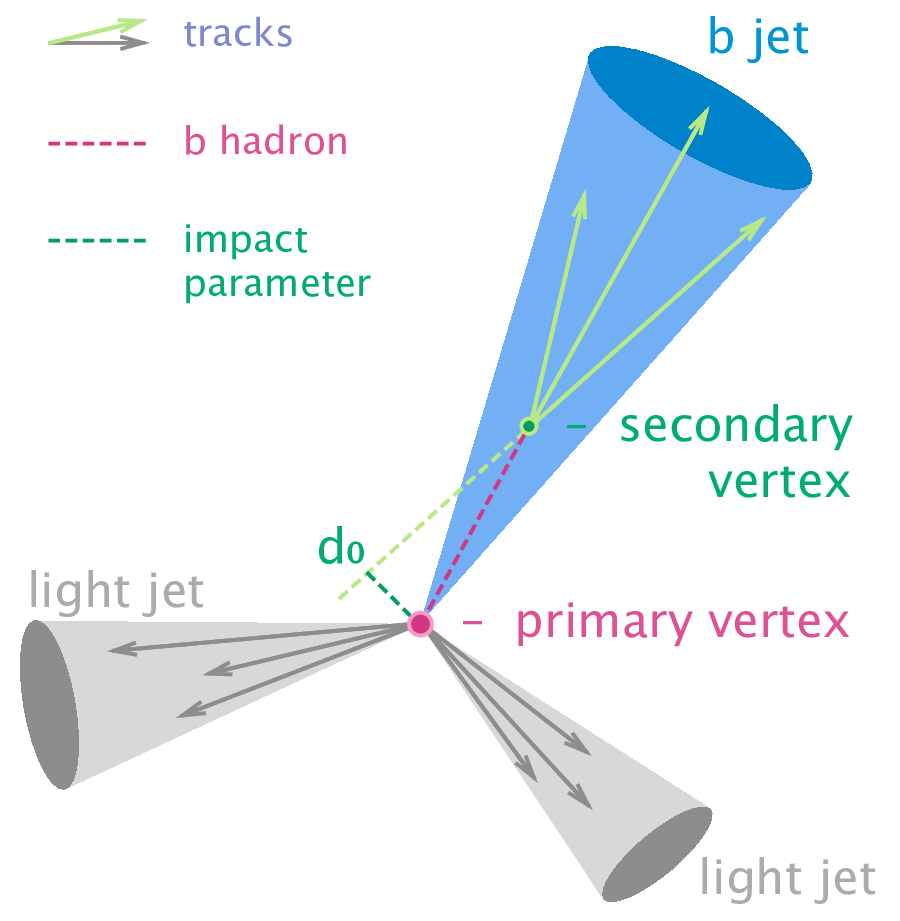
\includegraphics[width=0.25\textwidth]{chapters/3.tracking/figs/b-jet-diagram.png}
    \caption{Diagram of a typical \bjet (blue) which has been produced along with two light jets (grey). The \bhadron has travelled a significant distance from the primary interaction point (pink dot) before its decay. The large transverse impact parameter $d_0$ is a characteristic property of the trajectories of \bhadron decay products.}
    \label{fig:b-jet topology}
\end{figure}
%
At the LHC, $b$ quarks are generated in the hard scattering of proton-proton ($pp$) collisions. They quickly hadronize into a \bhadron, which is often initially in an excited state due to the high energies of the $pp$ collisions at the LHC ($\sqrt{s} = 13$ TeV). The hadronisation process is hard - around 70-80\% of the $b$ quark's momentum goes into the \bhadron, with the rest being radiated as other particles. The excited \bhadron will quickly fragment (i.e. de-excite) by radiating particles, which are prompt (they are formed closed to the primary vertex). These fragmentation particles have an increasing multiplicity and collimation to the \bhadron axis as the \pT of the \bhadron increases. The de-excited \bhadron subsequently weakly decays to $\sim 5$ particles (the multiplicity of the weak \bhadron decay products is unaffected by increases in the \bhadron \pT.). 

Due to their lifetimes, energetic \bhadrons can travel a significant distance from the primary $pp$ interaction point before decaying to a spray of collimated stable particles. This signature is registered in the detector as a displaced jet. Due to the elements of the CKM matrix, \bhadrons decay with a high probability to D hadrons (which contain a $c$ quark), which also have significant lifetimes - this can lead to reconstructed tertiary vertices in the jet core. The typical features of a \bjet, and in particular the large track impact parameter $d_0$ which can result from displaced decays, are shown in \cref{fig:b-jet topology}.
%
\begin{figure}[!htbp]
    \centering
    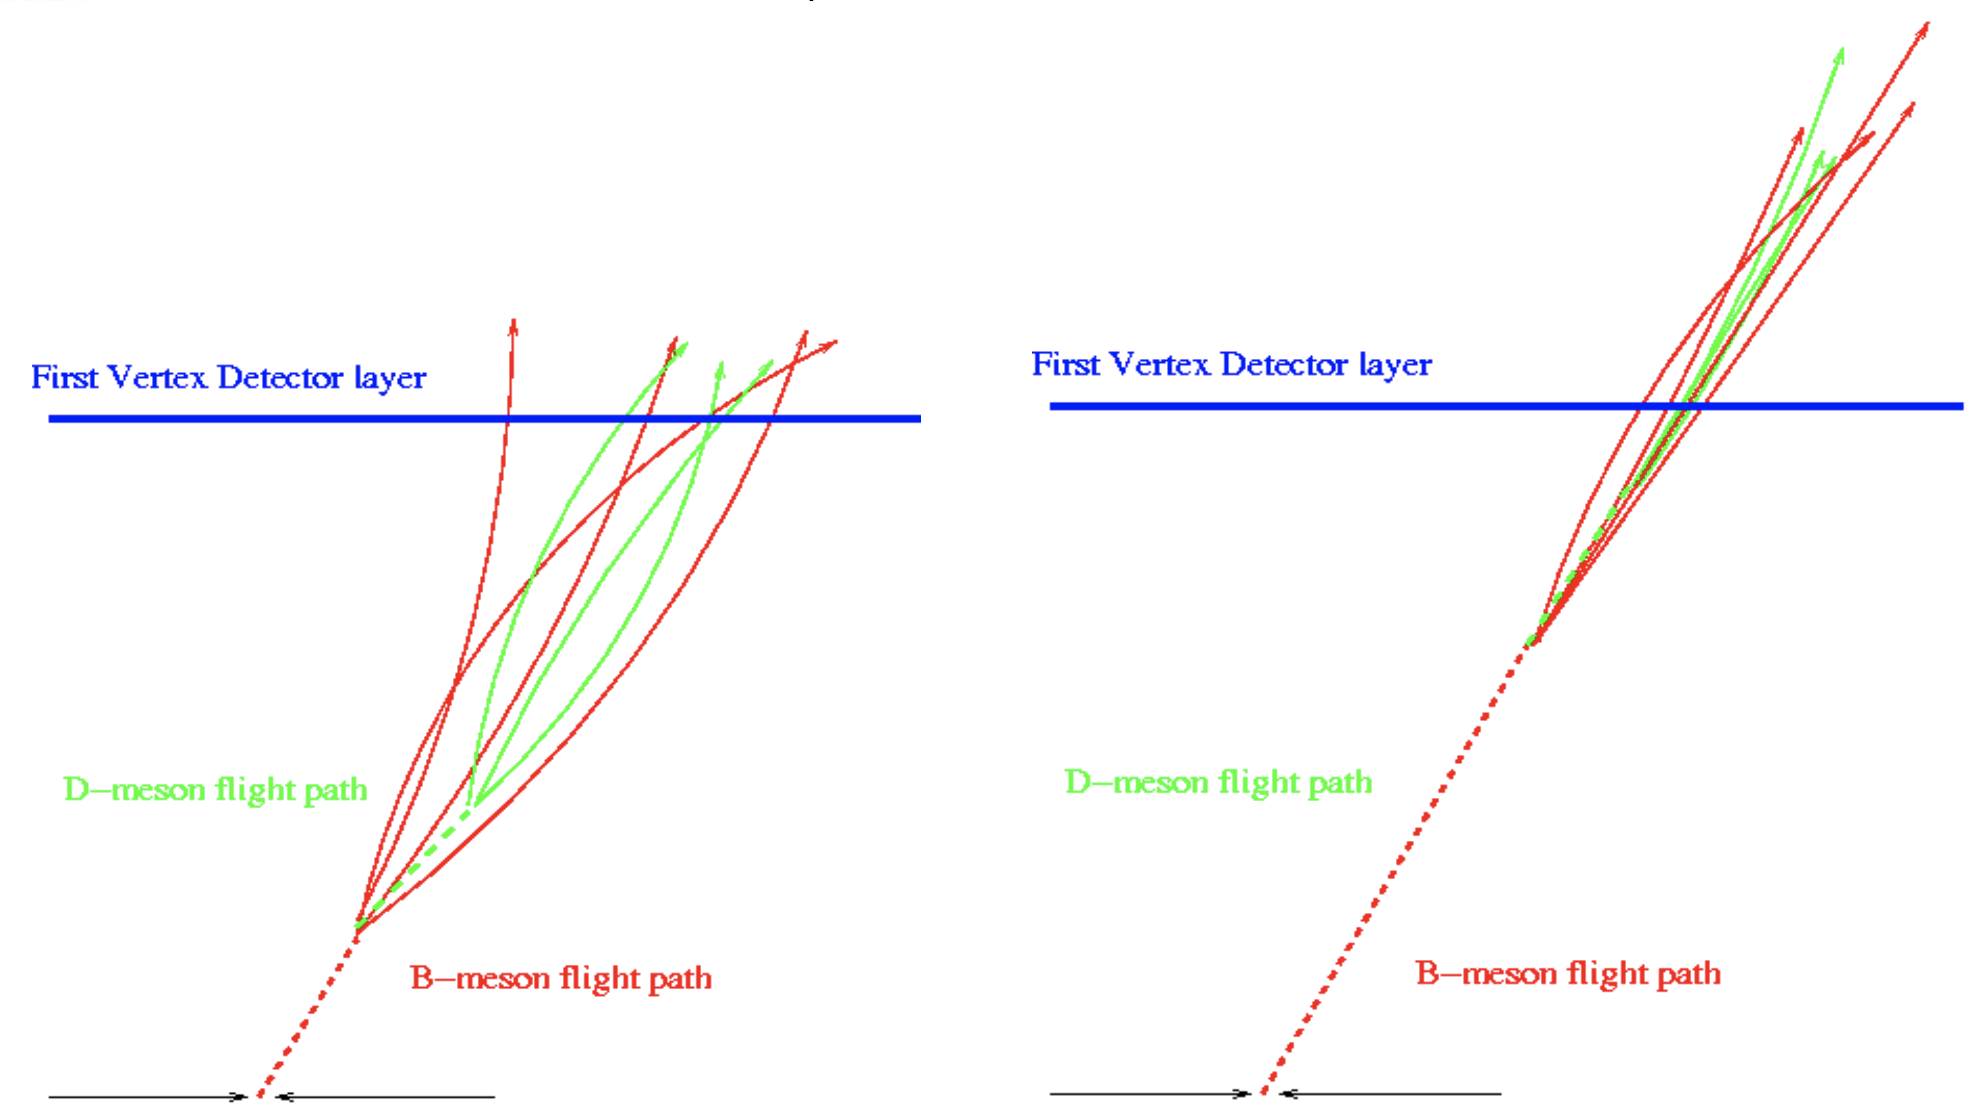
\includegraphics[width=0.7\textwidth]{chapters/3.tracking/figs/high-pt-b-tracks.png}
    \caption{As \bhadron $p_\text{T}$ increases, the time of flight of the B increases, so tracks will have less room to diverge before reaching detector elements. To compound the problem, the collimation of the tracks increases. The detector may then be unable to resolve individual tracks.}
    \label{fig:B hadron tracking problems}
\end{figure}
%
Many ATLAS analyses rely on a method of tagging jets instantiated by $b$ quarks and rejecting jets created from other quarks ($c$ and light flavours $u$, $d$, $s$). These ``\btagging'' algorithms work by discriminating against the unique signatures of \bjets discussed above. \btagging relies on the efficient and accurate reconstruction the tracks corresponding to the \bhadron decay products. These tracks are then used as inputs to vertex reconstruction algorithms and jet making algorithms.


\subsubsection{Reconstruction Challenges}\label{sec:B track reco challenges}

A necessary requirement for successful jet \btagging is the efficient and accurate reconstruction of the charged particle trajectories in the jet. For high \pT jets (\pT $> 200$ GeV) this task becomes difficult due to a combination of effects. As the jet energy increases, the track multiplicity of the jet increases due to the presence of additional fragmentation tracks. Tracks in the jet also become increasingly collimated as their inherited transverse momentum increases. Together, these two effects lead to a very high density of charged particles in the jet core, making reconstruction difficult. At high energies, the increased decay length of B (and D) hadrons means that decay products have less of an opportunity to diverge before reaching the first tracking layers of the detector. If the decay takes place very close to a detector layer, or if the decays are sufficiently collimated, hits left by nearby particles may not be resolved individually, leading to merged clusters (shown in \cref{fig:B hadron tracking problems}). Shared hits generally predict bad tracks. As such, shared hits are heavily penalised during reconstruction (and in particular as part of ambiguity solving). However, in the core of high \pT \bjets, where decay particles are displaced from the primary vertex and are highly collimated, the density of particles is high enough that the probability of clusters being merged increases dramatically. The presence of merged clusters requires that the corresponding tracks share hits (if they are to be reconstructed successfully), which may end up impairing the successfully reconstruction of the track. Furthermore, decays may also take place inside the tracking detectors themselves, which can lead to missing or wrong innermost cluster assignment. The combination of effects described above makes reconstructing tracks in the core of high \pT \bjets particularly challenging.


%
\begin{figure}[!htbp]
    \centering
    \begin{subfigure}{.5\textwidth}
      \centering
      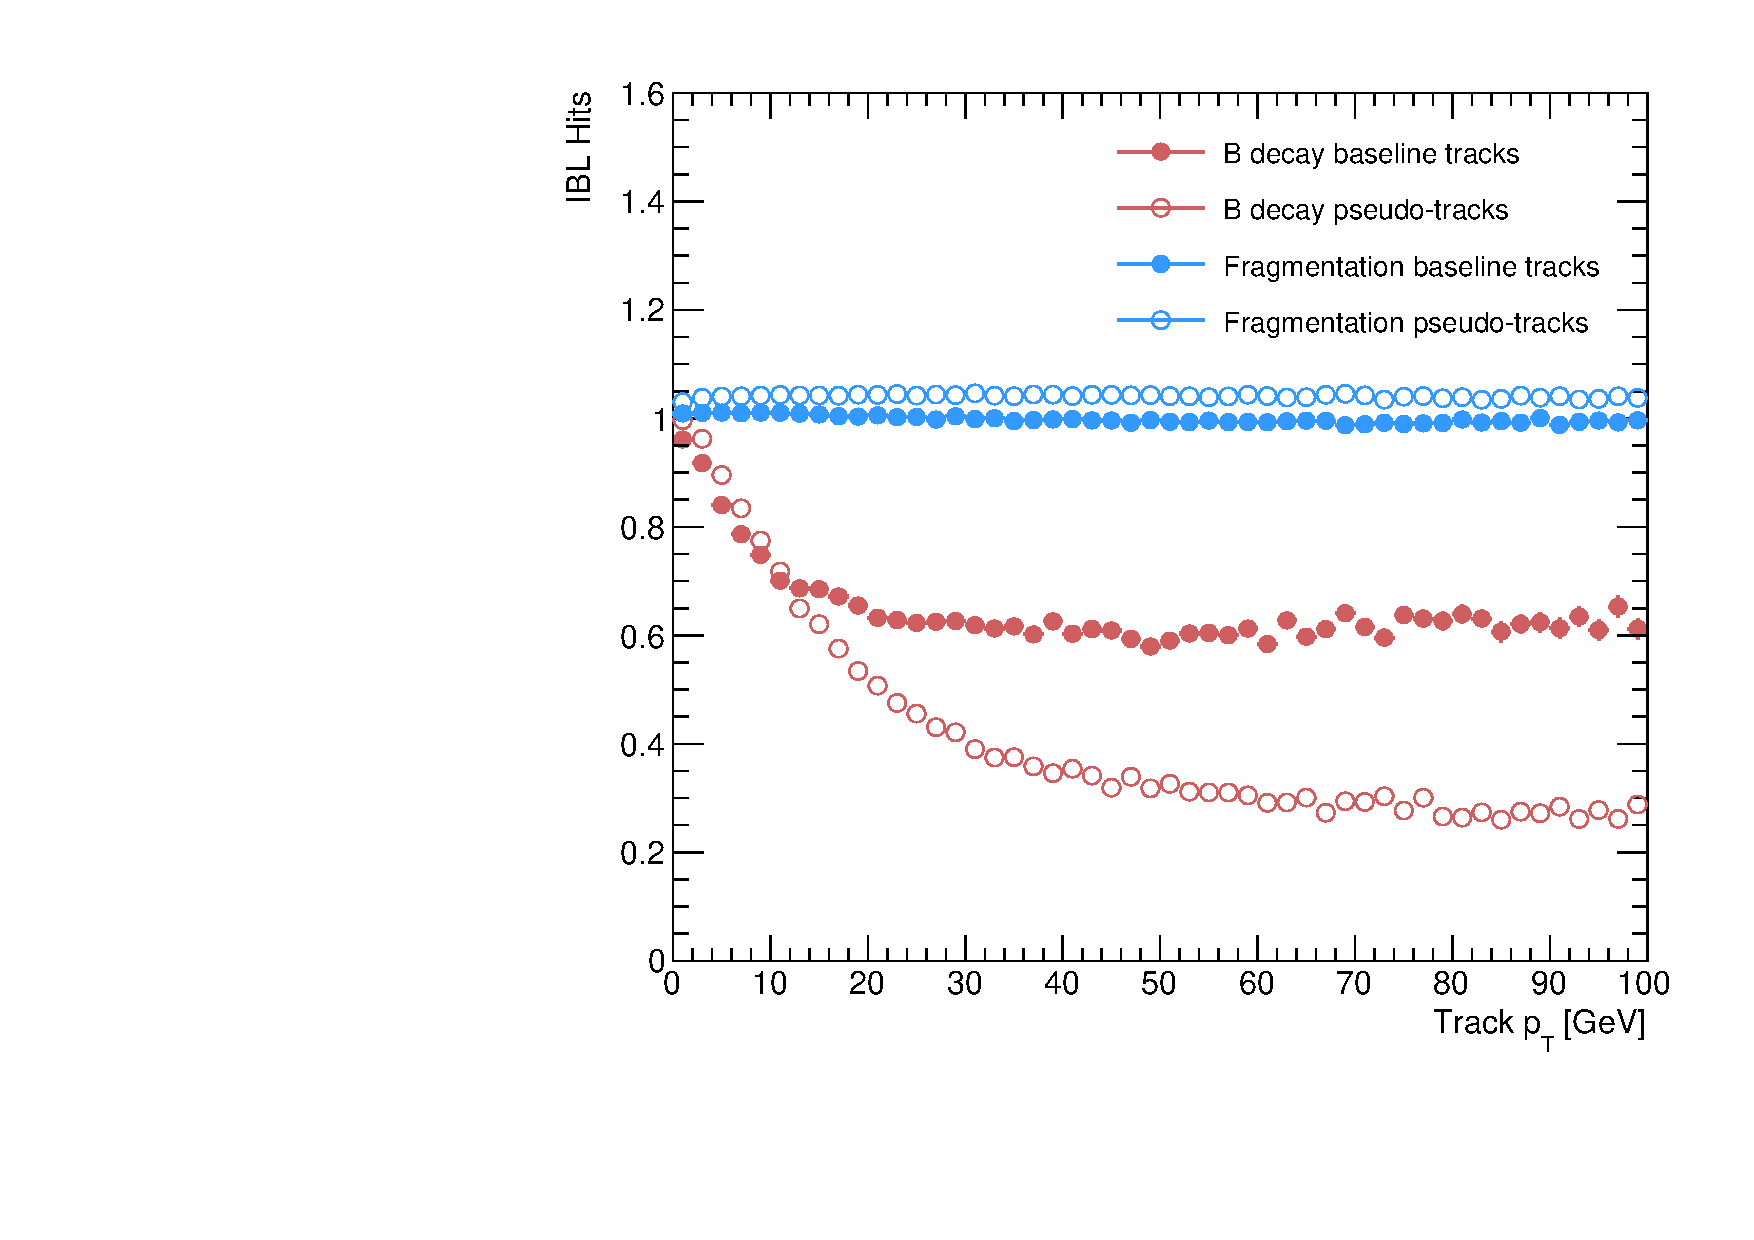
\includegraphics[width=\textwidth]{chapters/3.tracking/figs/overlay_po_nHitsOnIBL_From_B_pT.pdf}
      \caption{}
      \label{fig:n hits on ibl}
    \end{subfigure}%
    \begin{subfigure}{.5\textwidth}
      \centering
      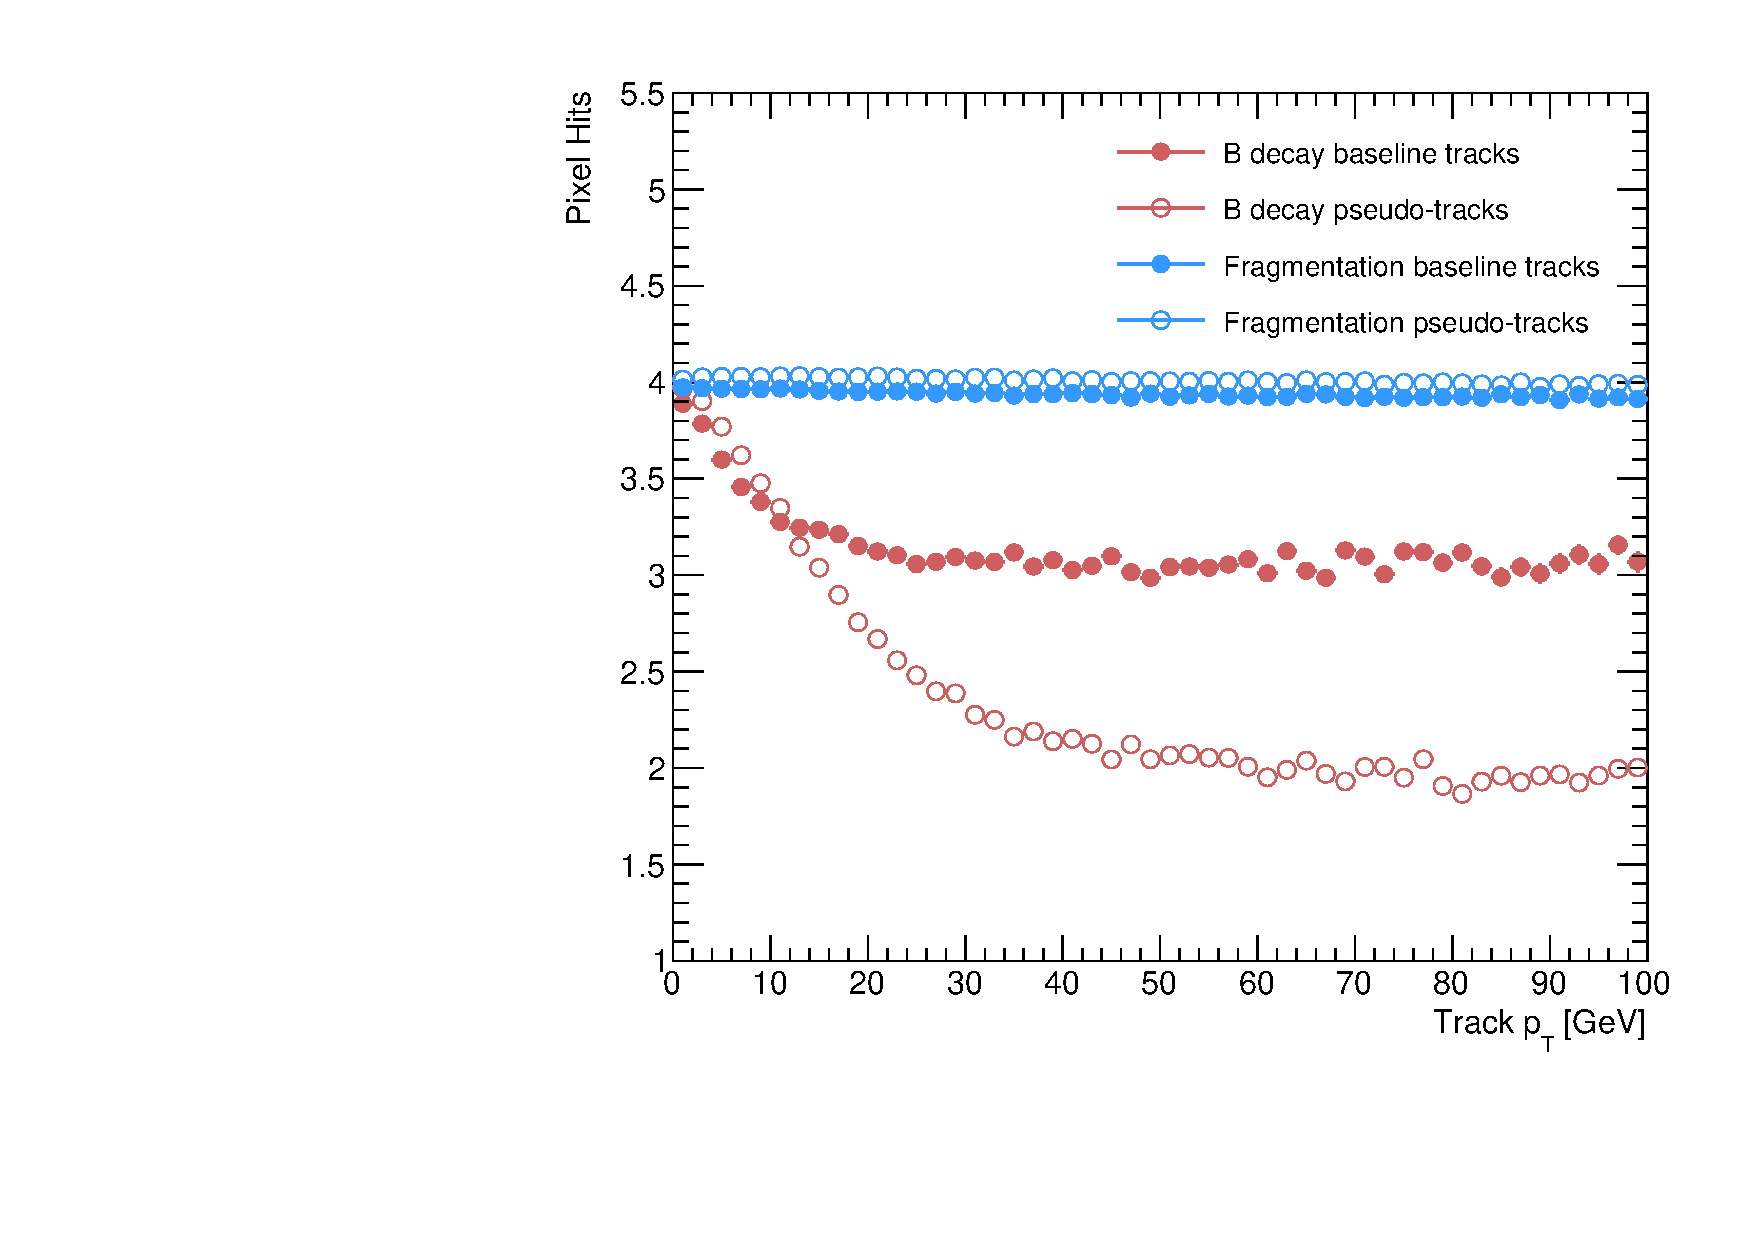
\includegraphics[width=\textwidth]{chapters/3.tracking/figs/overlay_po_nHitsOnPix_From_B_pT.pdf}
      \caption{}
      \label{fig:n hits on pix}
    \end{subfigure}
    \caption{Hit multiplicities on the IBL (\cref{fig:n hits on ibl}) and the all pixel layers (\cref{fig:n hits on pix}) as a function of the transverse momentum \pT of the reconstructed track. Tracks from the weak decay of the \bhadron are shown in red, while fragmentation tracks (which are prompt) are in blue. For each of these, standard tracks and pseudo-tracks are plotted. Hit multiplicities on the pseudo-tracks at high $p_\text{T}$ due to the increased flight of the \bhadron. The baseline tracks have more hits than the pseudo-tracks, indicating that they are being incorrectly assigned additional hits.}
    \label{fig:total hits on pix bs, frag}
\end{figure}
%







%
\begin{figure}[!htbp]
    \centering
    %\includegraphics[width=\textwidth]{res/figs/results/tracking/b-reco-efficiency.png}
    \vspace{0.05em}
    \caption{Track reconstruction efficiency from \bhadron decay products for baseline ATLAS tracking (black), Bcut+Refit procedures applied (green), pseudo-tracking (blue), and for tracking where the ambiguity solver has been manually removed (orange).}
    %The relatively high reconstruction efficiency at the stage of the track candidates (i.e. before ambiguity solving) indicates that the efficiency loss is driven by the ambiguity solver.
    \label{fig:reconstruction efficiency from B}
\end{figure}

\begin{figure}[!htbp]
    \centering
    %\includegraphics[width=\textwidth]{res/figs/results/tracking/po_nHitsOnPix_From_B_DL.pdf}
    \vspace{0.05em}
    \caption{The total number of pixel hits on tracks from \bhadron decays as a function of the production radius of the decay product. An excess of hits is assigned to the standard tracks in comparison to the ideal pseudo-tracks.}
    \label{fig:total hits on pix from b}
    \label{fig:misc}
\end{figure}
%

Concretely, then, the issues relating to high \pT \bhadron tracking can be factorised into two parts. The first part is a drop in track reconstruction efficiency. As mentioned, tracks originating from high energy \bhadron decay products can have a high rate of shared hits due to the number of particles present in a high \pT \bjet and their relative collimation. Additionally, tracks may be missing hits on the inner layers of the detector. This occurs primarily when the decay \bhadron decays inside the detector. These features of can make it difficult for B decay tracks to meet the ambiguity solver's stringent track quality requirements. As a result, many B decay tracks are rejected in the ambiguity solving stage, leading to a severe drop in tracking reconstruction efficiency. This is shown by the severe decrease in reconstruction efficiency visible when comparing baseline tracking with the ideal pseudo-tracks in \cref{fig:reconstruction efficiency from B}. This situation presents a problem: relaxing cuts on shared hits significantly degrades the ambiguity solver's power to reject bad tracks. However for \bhadron decay tracks it seems these same restrictions on shared hits are seriously impairing the reconstruction efficiency of good tracks. The second part of the problem is that, due to the high density of clusters available for assignment in the vicinity of the typical high energy \bhadron decay track, and also given the strong positive bias of the ambiguity solver towards those tracks with precise pixel measurements (especially the innermost IBL measurement), many \bhadron decay tracks are assigned incorrect inner layer hits. This is only a problem for those decay products which were produced inside the pixel detector as a result of a long-flying \bhadron, and so do not have a correct hit available for assignment (evidenced in \cref{fig:refit optimisation results sub2}). The incorrect hits may skew the parameters of the track, which can in turn mislead \btagging algorithms. In particular, \btagging algorithms rely heavily on the transverse impact parameter significance $d_0/\sigma(d_0)$ of the track. The quality of this measurement is expected to be adversely affected by wrong inner-layer hits on the track. This combination of reduced reconstruction efficiency and incorrectly assigned hits is thought to be the cause of the observed drop in \btagging efficiency at high energies , although it is not clear which effect may dominate.


\subsection{Pseudotracks and Ideal Tracks}\label{sec:pseudo ideal tracking}

Pseudotracking and ideal tracking are used as benchmarks of the best tracking possible given the ATLAS detector. Both pseudotracks and ideal tracks are constructed using truth information to group combinations of hits that have been left by the same truth particle. As a result, hit-to-track association and track reconstruction efficiency are both ideal (given the ATLAS detector). Ideal tracks represent a yet more idealised tracking scenario by correcting the cluster positions based on truth information, and smearing the cluster position based on the detector resolution.

When pseudotracking is run alongside standard tracking, those clusters which are shared on the reconstructed tracks run through the cluster splitting machinery. If a cluster is found to be compatible with being split, its definition is changed, and the pseudotracks use this definition too. As a result, pseudotracks can have split clusters.


\section{Track Labelling}\label{sec:track labelling}

\subsection{B Tracks}\label{sec:B track labelling}
\subsection{Fake Tracks}\label{sec:fake track labelling}

\section{Investigating Improvements for High \texorpdfstring{\pT}{pT} B Tracking}\label{sec:investigating tracking improvements}

An investigation into

\subsection{TrackAnalysis Package}\label{sec:track analysis package}
\subsection{Looser Track Cuts \& Refit Procedure}\label{sec:bcut and refit}
\subsection{GX2F Outlier Removal}\label{sec:gx2f outlier removal}

